
\newpage

\begin{longtable}[]{@{}rrrrl@{}}
\caption{\label{tab:Tab1}A caption.}\tabularnewline
\toprule
Sepal.Length & Sepal.Width & Petal.Length & Petal.Width &
Species\tabularnewline
\midrule
\endfirsthead
\toprule
Sepal.Length & Sepal.Width & Petal.Length & Petal.Width &
Species\tabularnewline
\midrule
\endhead
5.1 & 3.5 & 1.4 & 0.2 & setosa\tabularnewline
4.9 & 3.0 & 1.4 & 0.2 & setosa\tabularnewline
4.7 & 3.2 & 1.3 & 0.2 & setosa\tabularnewline
4.6 & 3.1 & 1.5 & 0.2 & setosa\tabularnewline
5.0 & 3.6 & 1.4 & 0.2 & setosa\tabularnewline
\bottomrule
\end{longtable}

\newpage

\begin{figure}[h]

{\centering 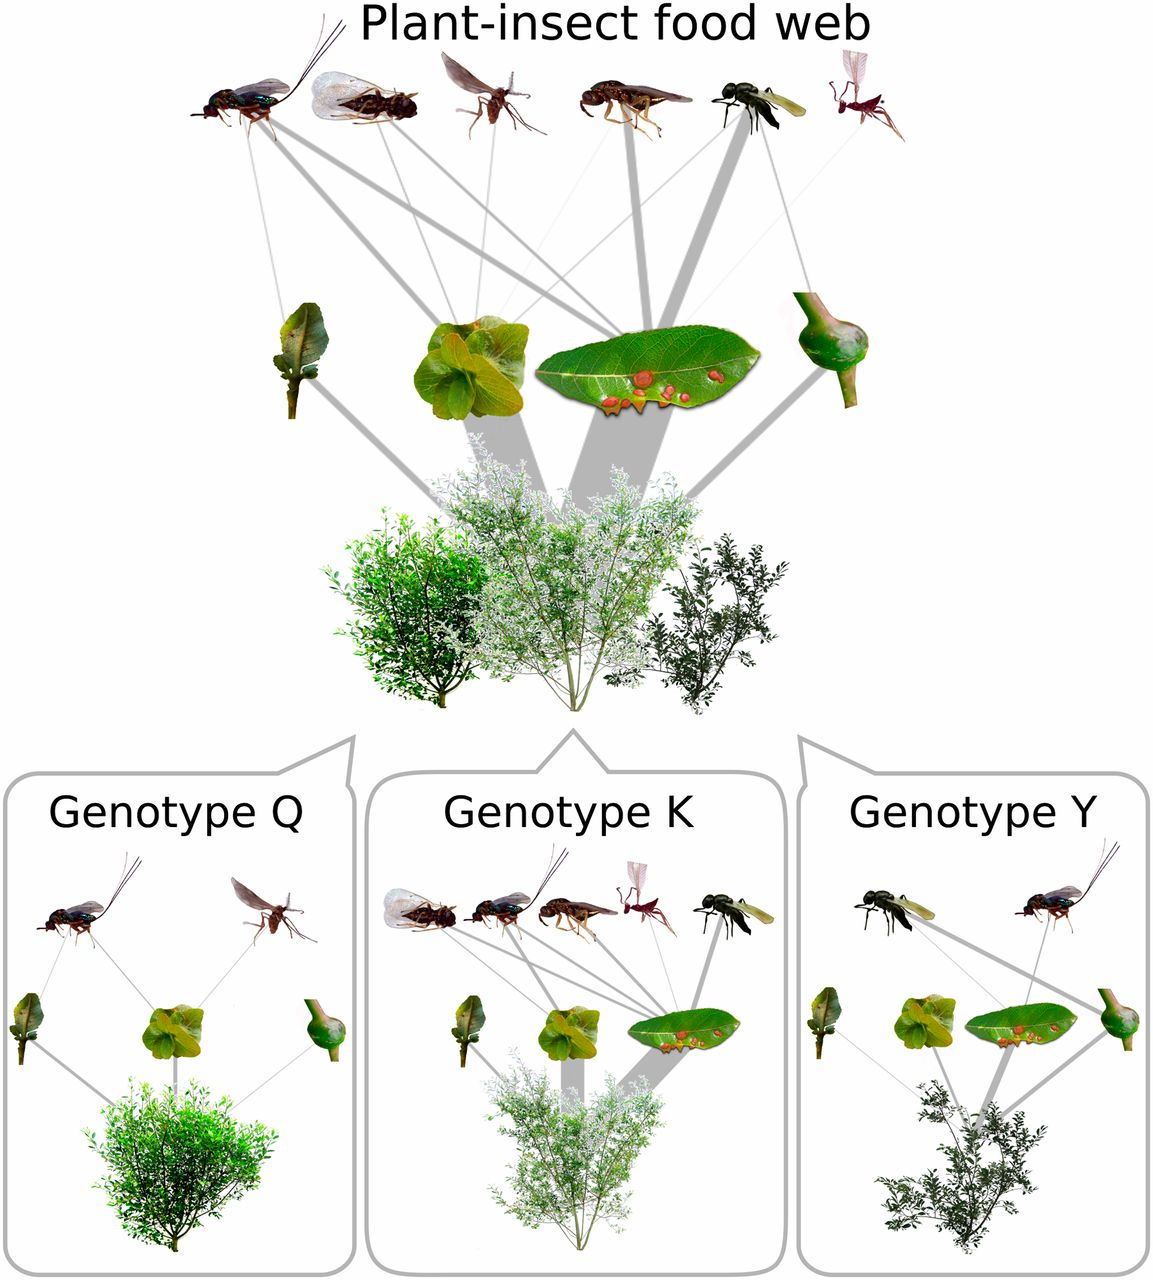
\includegraphics[width=0.5\linewidth]{Figures/F1.large} 

}

\caption{\label{fig:Fig1}Here is a nice figure from one of my papers. You can use chunk options for resizing and aligning the figure.}\label{fig:ChunkName}
\end{figure}

\newpage

\begin{figure}
\centering
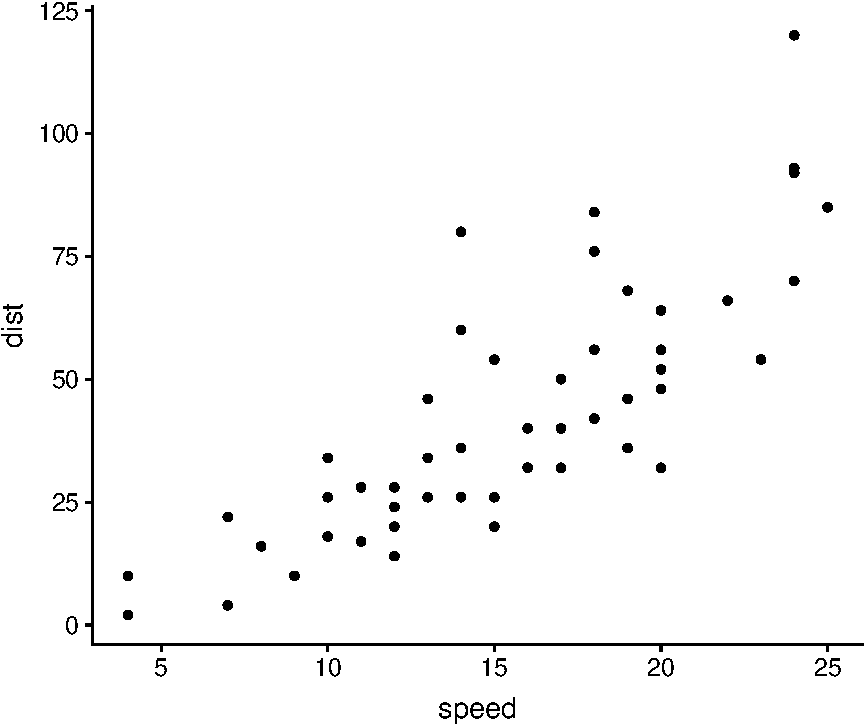
\includegraphics{Figures_AfterBody_files/figure-latex/Rplot-1.pdf}
\caption{\label{fig:Fig2}Here is a figure generated directly from R
code. Note that you use different chunk options to adjust this type of
figure.}
\end{figure}



